Agora que sabemos como criar uma gema, visto no capítulo \ref{chapter:criacao_de_bibliotecas_do_ruby},
podemos partir para a ideia de fazer modificações em uma gema que já existe, ou seja, fazer a adição
de novas funcionalidades com base em uma gema já existente.

Suponha o cenário aonde utilizamos com frequência uma certa gema, no entanto apesar dela comportar várias
funcionalidades, ela não possui tudo que desejamos. Neste caso, basta fazer a adaptação desta gema, não
sendo necessário criar uma nova gema do zero.

Este capítulo tem o objetivo de mostrar os passos que devem ser realizados para se adaptar uma
biblioteca do \emph{Ruby}. Na seção \ref{section:modelo_de_adaptação}, apresentaremos o modelo de adaptação
que deve ser seguido para adaptar um gema, e depois apresentaremos na seção \ref{section:exemplo_de_adaptação},
um exemplo da adaptação de uma gema que mapeia a \emph{API} do \emph{Google Maps}.


\section{Modelo de Adaptação}
\label{section:modelo_de_adaptação}


Como citado anteriormente, o primeiro passo é encontrar uma gema que atenda boa parte das nossas
necessidades e que utilizamo com frequência. Nesse passo, depois de determinar a gema a ser adaptada,
devemos tomar cuidado ao adicionar qualquer funcionalidade nela, pois podemos estar comprometendo o
contexto da gema, ou seja, comprometendo o objetivo final da biblioteca.

Para não comprometer o objetivo final da gema, é sempre válido verificar se a funcionalidade
que estamos adicionando, esta no mesmo contexto da gema. Pois por exemplo em uma biblioteca matemática,
podemos adicionar uma função para calcular a raiz quadrada. No entanto por outro lado,
não faz nenhum sentido incluir uma funcionalidade de criar mapas do \emph{Google} nesta biblioteca,
pois esta funcionalidade de mapas não está no mesmo contexto da biblioteca.

Nesta seção apresentaremos na seção \ref{subsection:engenharia_reversa} o processo de engenharia
reversa para transformar um sistema em diagramas de alto nível, depois na seção
\ref{subsection:entendimento_da_biblioteca}, apresentaremos uma forma para fazer a leitura dos
diagramas de alto nível, e por fim apresentaremos na seção \ref{subsection:adaptações}, o processo
de adaptação.


\subsection{Engenharia Reversa}
\label{subsection:engenharia_reversa}


Esta seção tem o objetivo de apresentar a importância da \emph{engenharia reversa} no processo de adaptação
de uma gema. Inicialmente veremos uma definição do processo de \emph{engenharia reversa}.

Para conseguirmos entender o funcionamento de uma gema, precisamos obrigatoriamente fazer uma tradução
do código fonte para diagramas, pois não conseguiremos fazer nenhuma modificação consistente
se não tivermos uma visão geral de seu funcionamento, e esse procedimento de tradução se chama
\emph{engenharia reversa}.

A \textbf{\emph{engenharia reversa}} é um processo de análise para a extração de informações de algo que já
existe em um modelo de abstração de alto nível. Essas informações podem estar no formato de código
fonte ou mesmo em um executável. O processo de análise para a extração de dados deve ser feita de forma
minuciosa, pois caso alguma funcionalidade seja entendida de forma incorreta, existe a possibilidade de
perda de recursos. E o modelo de abstração de alto nível, pode ser por exemplo um diagrama de classe
ou um diagrama de herança.


\subsection{Entendimento da Biblioteca}
\label{subsection:entendimento_da_biblioteca}


Agora que realizamos a \emph{engenharia reversa} da \emph{gema} para construir os diagramas
de alto nível na seção \ref{subsection:engenharia_reversa}. Devemos fazer a anaĺise destes
diagramas para identificar os elementos do sistema, como por exemplo, classes e componentes.

Após a identificação dos elementos, devemos verificar para que cada um deste elemento é utilizado, ou seja,
verificar o motivo pelo qual, determinado elemento existe no sistema.

Também devemos verificar quais são os principais elementos. Neste caso, os principais elementos
são aqueles que são indispensáveis para o funcionamento da gema. Como por exemplo, o objeto mapa
é um elemento indispensável para mostrar um mapa na tela.

Depois de fazer a identificação dos elementos, passamos para a parte de análise das funcionalidades.
Nesse passo, verificamos quando os elementos são criados e em quais funcionalidades eles são utilizados.

Desta forma com a identificações dos elementos e das funcionalidades, temos um entendimento completo da
biblioteca.


\subsection{Adaptações}
\label{subsection:adaptações}


Esta seção tem o objetivo de apresentar como podemos fazer adaptações nas gemas, após realizar o
processo de \emph{engenharia reversa} e o processo de entendimento da biblioteca.

Inicialmente devemos verificar se é necessário fazer a inclusão de novos elementos, pois com já sabemos
quais os elementos existentes no sistema, e o motivo pelo qual eles existem, podemos analisar se é ou não
necessário incluir novos elementos.

Depois da análise da inclusão de novos elementos, devemos verificar quais os elementos que vão receber
as novas funcionalidades, sempre verificando se não estamos modificando o objetivo final do elemento.

Por fim, após fazer a análise dos elementos e das funcionalidade, devemos considerar os impactos das modificações,
verificando se nenhuma funcionalidade, já existente, foi afetada.


\section{Exemplo de Adaptação}
\label{section:exemplo_de_adaptação}


O objetivo desta seção é apresentar um exemplo da adaptação da gema
\emph{\href{https://github.com/apneadiving/Google-Maps-for-Rails}{Google-Maps-for-Rails}}
\footnote{Google-Maps-for-Rails : \url{https://github.com/apneadiving/Google-Maps-for-Rails}} criada por
\emph{\href{https://github.com/apneadiving}{Benjamin Roth}}
\footnote{Bejamin Roth: \url{https://github.com/apneadiving}} e
\emph{\href{https://github.com/MrRuru}{David Ruyer}} \footnote{David Ruyer: \url{https://github.com/MrRuru}}.
Essa gema tem como objetivo criar mapas de forma simplificada, proporcionando a inclusão de
sobreposições oferecidas pelo \emph{Google}, como por exemplo, marcadores e círculos. Ela também possui
um código flexível que permite a aceitação de outros provedores de mapas, como por exemplo o
\emph{Bing Maps} [\citeonline{google_maps_for_rails}].

Na seção \ref{subsection:google_maps}, apresentaremos alguns conceitos da \emph{API} do
\emph{Google}. Em seguida na seção \ref{subsection:coffeescript}, apresentaremos alguns conceitos da linguagem
\emph{CoffeeScript}, linguagem utilizada na gema para mapear a \emph{API} do \emph{Google Maps}. Depois na
seção \ref{subsection:abordagem_de_adaptacao}, apresentaremos a abordagem utilizada para adaptar a gema. Em
seguida apresentaremos na seção \ref{subsection:engenharia_reversa_da_biblioteca_de_exemplo}, a realização
do processo de \emph{engenharia reversa} na gema de exemplo. Depois na seção
\ref{subsection:entendimento_da_biblioteca_adaptada}, apresentaremos um análise dos elementos da gema
‘‘\emph{Google-Maps-for-Rails}''. Em seguida na seção \ref{subsection:adaptações_da_biblioteca_de_exemplo},
apresentaremos as modificações realizadas na gema de exemplo. E por fim apresentaremos na seção
\ref{subsection:exemplo_de_uso_da_biblioteca_adaptada}, um exemplo do uso de ‘‘\emph{Google-Maps-for-Rails}''
em um projeto do \emph{Ruby On Rails}.


\subsection{Google Maps}
\label{subsection:google_maps}


Para fazer a adaptação da gema foi necessário fazer um estudo sobre como utilizar a \emph{API} do
\emph{Google} e para isso foi utilizado como base o livro \emph{Beginning Google Maps API 3}
[\citeonline{beginning_google_maps_api3}] e a
\emph{\href{https://developers.google.com/maps/}{Google Maps API V3}}
\footnote{Google Maps API V3: \url{https://developers.google.com/maps/}}, onde ambos se complementam
ensinando os passos básicos para criar e manipular mapas do \emph{Google} utilizando \emph{Javascript}.

O \emph{Google Maps} e sua respectiva \emph{API} foram criadas por dois irmãos \emph{Lars} e
\emph{Jens Rasmussen}, cofundadores da ‘‘\emph{Where 2 Technologies}'', companhia dedicada a criação de mapas
que foi comprada pelo \emph{Google} em 2004 [\citeonline{beginning_google_maps_api3}].

Antes de criação do \emph{Google Maps}, existia um grande problema de renderização que ocorria por causa
que um mapa era um elemento único. Devido a este fato, podemos perceber que o elemento do mapa
possuía uma grande quantidade de informações. Deste modo, fica claro que a transferência de um mapa entre
um servidor e um cliente, era uma tarefa cara, pois era necessário fazer a transferência de uma grande
quantidade de dados. E além de existir uma alto custo na transferência, também existia um alto custo no
cliente no momento da transformação das informações em forma de mapa.

O \emph{Google Maps} fez a divisão dos mapa em vários pedaços, uma vez que o problema da renderização
ocorria por causa da representação do mapa em um elemento único
[\citeonline{google_maps_power_tools_for_maximizing_the_api}]. Nesta solução, os pedaços dos mapas
poderiam ser requisitados um a um para montar uma parte ou um mapa completo. Desta forma, foi possível
solucionar o problema da grande quantidade de dados transferidos, pois somente se transfere as partes
requisitadas do mapa, e também se solucionou o problema da transformação, pois a quantidade de dados
para se transformar, foi reduzida razoavelmente.

A ferramenta \emph{Google Maps} manipula mapas por meio de \emph{HTML}, \emph{CSS} e \emph{Javascript}.
O posicionamento dos mapas é feito por meio de \emph{HTML} e \emph{CSS}. As requisições e o posicionamento
dos pedaços dos mapas são feito por meio de \emph{Javascript}.

O processo de manipulação de mapas possui 3 etapas. Na primeira, o usuário por meio do \emph{browser},
requisita algum local do mapa informando a coordenada e o zoon desejado. Na segunda, o servidor recebe
a requisição, procura o pedaço, e retorna a imagem do mapa que representa a posição requisitada. Na
terceira, o \emph{browser} recebe e renderiza a imagem no mapa [\citeonline{beginning_google_maps_api3}].


\subsection{CoffeeScript}
\label{subsection:coffeescript}


Para fazer a adaptação da gema, também foi necessário fazer um estudo sobre a linguagem
\emph{\href{http://coffeescript.org/}{CoffeeScript}}, pois ela é utilizada na gema para
mapear a \emph{API} do \emph{Google Maps}.

O \emph{CoffeeScript} é uma linguagem que simplifica o modo de desenvolver códigos \emph{Javascript},
expondo os melhores pontos de forma simples e clara. A regra de ouro do \emph{CoffeeScript}
é que ‘‘\emph{CoffeeScript é simplesmente Javascript}'', pois o seu código é compilado linha a linha,
sendo transformado em \emph{Javascript} [\citeonline{coffeescript_site}].

A linguagem permite o uso de qualquer biblioteca escrita em \emph{Javascript}. Seu código compilado,
é legivel e identado, podendo executar em um tempo superior ao de um código \emph{Javascript} escrito
manualmente [\citeonline{coffeescript_site}].

Vimos na seção \ref{subsection:google_maps} que a \emph{API} do \emph{Google Maps} funciona sobre
\emph{Javascript}. Como o \emph{CoffeeScript} é \emph{Javascript}, e já que o seu desenvolvimento
é mais simples. Ele foi utilizado para mapear a \emph{API} do \emph{Google Maps} na gema original
e na adaptada.


\subsection{Abordagem de Adaptação}
\label{subsection:abordagem_de_adaptacao}


Para realizar as adaptações na gema \emph{Google-Maps-For-Rails}, vamos seguir o modelo de adaptação,
visto na seção \ref{section:modelo_de_adaptação}.

Nas seções seguintes, vamos realizar o processo de engenharia reversa, o entendimento, e as adaptações
na gema. Alguns conceitos do processo de engenharia reversa e o entendimento da gema, já foram vistos
nas seções \ref{subsection:engenharia_reversa} e \ref{subsection:entendimento_da_biblioteca},
respectivamente. Para realizar as adaptações, poderiamos utilizar uma entre duas abordagens.

A primeira consiste em criar uma nova biblioteca que inclui a biblioteca original e acrescenta novas
funcionalidades. Neste caso deveriamos criar uma nova biblioteca, importar a biblioteca original, e
adicionar novas funcionalidades. A vantagem desta abordagem é que a nova biblioteca sempre receberá
as atualizações feitas na biblioteca original.

A segunda consiste em criar uma nova biblioteca, copiar todo código da biblioteca original e acrescentar
novas funcionalidades. Neste caso deveriamos criar um \emph{branch} da biblioteca original e adicionar
novas funcionalidades. A vantagem desta abordagem é que a nova biblioteca é independente da biblioteca
original.

Acabamos optando pela segunda abordagem, pois mudanças na biblioteca original, poderiam causar
transtornos nas modificações, prejudicando assim o desenvolvimento deste trabalho.


\subsection{Engenharia Reversa da Biblioteca de Exemplo}
\label{subsection:engenharia_reversa_da_biblioteca_de_exemplo}


Aplicando a \emph{engenharia reversa} na gema \emph{Google-Maps-For-Rails}, conseguimos obter como resultado
O diagrama de atributos na imagem \ref{fig:diagrama_de_atributos_google_maps_for_rails} que possui as classes
e os seus respectivos atributos. 3 diagramas de métodos na imagem
\ref{fig:diagrama_de_metodos_google_maps_for_rails} que possui as classes e os seus respectivos métodos.
O diagrama de herança na imagem \ref{fig:diagrama_de_heranca_google_maps_for_rails} que possui apresenta a
heraça entre as classes.

Nenhum dos 3 diagramas existe na definição de diagramas da \emph{UML}, e isso se deve ao fato de não
existir espaço suficiente na imagem para representar o sistema da gema por completo em um diagrama de classes.
Por esse motivo, optamos por definir novos diagramas que possuem características similares aos padrões da
\emph{UML}, mas com algumas representações adicionais, podendo assim representar o diagrama de classe por
completo.


\begin{figure}[ht]
  \begin{center}
    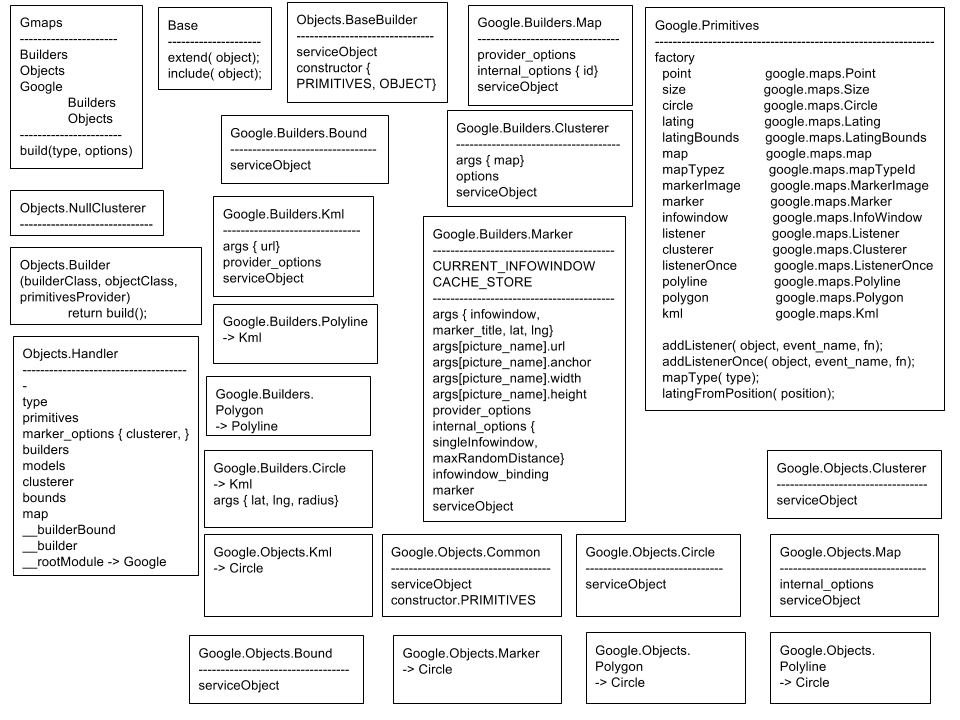
\includegraphics[scale=0.35]{images/diagrama_de_atributos_google_maps_for_rails.png}
    \caption{Diagrama de Atributos Google-Maps-For-Rails}
    \label{fig:diagrama_de_atributos_google_maps_for_rails}
  \end{center}
\end{figure}


As seguintes explicações são válidas para o diagrama de atributos apresentado na imagem
\ref{fig:diagrama_de_atributos_google_maps_for_rails}:

\begin{itemize}

 \item Todos os nomes abaixo do traço ‘‘-----'' representam os atributos da classe. Também
 existe o caso onde esse métodos são seguidos pelos símbolos ‘‘\{ ... \}'', onde o método é um
 \emph{objeto} e os nomes separados por ‘‘,'' entre os símbolos ‘‘\{ ... \}'' são os atributos
 do \emph{objeto}.

 \item Existem classes que não possuem os traços ‘‘-----'', neste caso elas possuem o nome delas
 seguida do símbolo ‘‘->'' e depois um nome de outra classe. Isso significa que esta classe
 possui os mesmo atributos da classe que vem depois do símbolo ‘‘->''. Por exemplo a
 classe ‘‘\emph{Google.Builder.Polyline -> Kml}'' que representa a classe
 ‘‘\emph{Google.Builder.Polyline}'', ela possuí os mesmo atributos da classe
 ‘‘\emph{Kml}'', ou seja, ela possuí os atributos
 ‘‘\emph{args \{ url \}}'', ‘‘\emph{provider\_option}'' e ‘‘\emph{serviceObject}''. E também existe o caso
 onde esta classe possuí atributos além dos da outra classe e nesse caso esses
 atributos são colocados na linha de baixo. Por exemplo a classe
 ‘‘\emph{Google.Builder.Circle -> Kml}'' que é a classe ‘‘\emph{Google.Builder.Circle}'', além de
 possuír os atributos da classe \emph{Kml}, ela possuí o atributo
 ‘‘\emph{args \{ lat, lng, radius \}}''.

\end{itemize}


\begin{figure}[ht]
  \begin{center}
    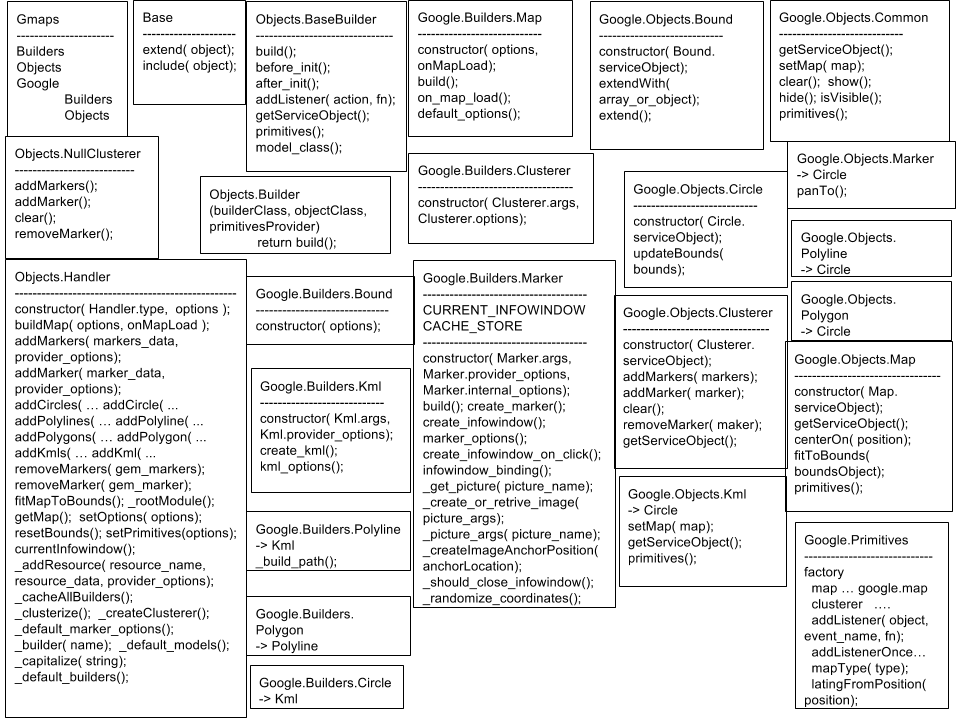
\includegraphics[scale=0.35]{images/diagrama_de_metodos_google_maps_for_rails.png}
    \caption{Diagrama de Métodos Google-Maps-For-Rails}
    \label{fig:diagrama_de_metodos_google_maps_for_rails}
  \end{center}
\end{figure}


As seguintes explicações são válidas para o diagrama de métodos na imagem
\ref{fig:diagrama_de_metodos_google_maps_for_rails}:

\begin{itemize}

 \item Todos os nomes seguidos de ‘‘(...)'' abaixo do traço ‘‘-----'' representam os métodos da classe.

 \item Existem classes que não possuem os traços ‘‘-----'', neste caso elas possuem o nome delas
 seguida do símbolo ‘‘->'' e depois um nome de outra classe. Isso significa que esta classe
 possui os mesmo métodos da classe que vem depois do símbolo ‘‘->''. Por exemplo a
 classe ‘‘\emph{Google.Builder.Circle -> Kml}'' representa a classe ‘‘\emph{Google.Builder.Circle}''
 e ela possuí os mesmo métodos da classe ‘‘\emph{Kml}'', ou seja, ela possuí os métodos
 ‘‘\emph{constructor()}'', ‘‘\emph{create\_...()}'' e ‘‘\emph{...\_option()}''. E também existe o caso
 onde esta classe possuí métodos além dos da outra, e nesse caso esses métodos são colocados na linha
 de baixo. Por exemplo a classe ‘‘\emph{Google.Builder.Polyline -> Kml}'' que é a classe
 ‘‘\emph{Google.Builder.Polyline}'', além de possuír os métodos da classe \emph{Kml}, ela
 possuí o método ‘‘\emph{\_build\_path()}''.

\end{itemize}


\begin{figure}[ht]
  \begin{center}
    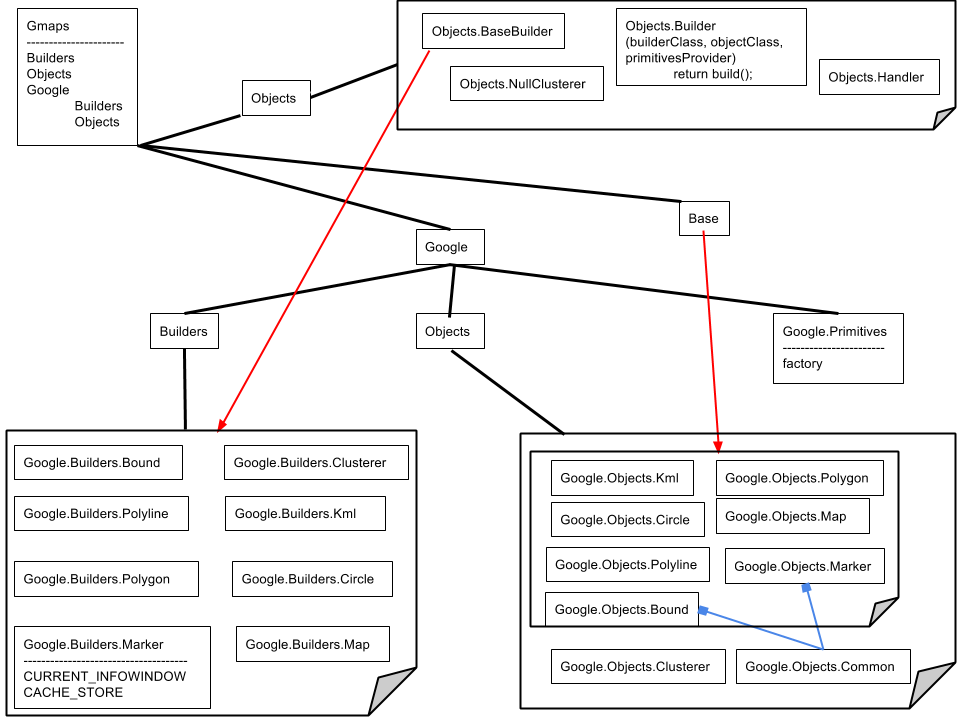
\includegraphics[scale=0.35]{images/diagrama_de_heranca_google_maps_for_rails.png}
    \caption{Diagrama de Herança Google-Maps-For-Rails}
   \label{fig:diagrama_de_heranca_google_maps_for_rails}
  \end{center}
\end{figure}


As seguintes explicações são válidas para o diagrama de herança na imagem
\ref{fig:diagrama_de_heranca_google_maps_for_rails}:

\begin{itemize}

 \item As linhas pretas continuas, indicam a organização da gema, sendo que a classe \emph{Gmaps}
 é a classe principal.

 \item Os retângulos normais representam as classes.

 \item A classe \emph{Gmaps} possui os atributos \emph{Builders}, \emph{Objects} e
 \emph{Google}, onde o \emph{Google} possui os atributos \emph{Builders} e \emph{Objects}.

 \item As linhas pretas em traços com pontas de seta, representam a herança entre duas
 \emph{classes}. A classe que está com a seta, é a classe que herda as características da classe
 na outra ponta da linha.

 \item As linhas pretas em pontos com pontas de quadrado, representam a inclusão de uma classe na outra.
 A classe que está com o quadrado, é a classe que incluí a classe que está na outra ponta da linha.

  \item Os retângulos que tem uma dobra no canto inferior direito, representam um conjunto de classes,
 onde estas classes possuem uma característica em comum. Por exemplo as classes ‘‘\emph{Kml}'',
 ‘‘\emph{Polygon}'', ‘‘\emph{Polyline}'', ‘‘\emph{Circle}'', ‘‘\emph{Map}'', ‘‘\emph{Marker}'' e
 ‘‘\emph{Bound}'' que são ‘‘\emph{Objects}'' do ‘‘\emph{Google}'', estão em um conjunto onde todas elas
 herdam as características da classe ‘‘\emph{Base}''.

 \end{itemize}


\subsection{Entendimento da Biblioteca Adaptada}
\label{subsection:entendimento_da_biblioteca_adaptada}


Para a gema de exemplo, seguindo o modelo de entendimento visto no capítulo anterior na seção
\ref{subsection:entendimento_da_biblioteca}, encontramos as seguinte características que serão
listadas e explicadas a seguir.

\begin{itemize}

 \item Apesar do ‘‘\emph{GMaps}'' ser a classe principal da gema, ela não é a mais
 importante, pois todas as funcionalidades da gema são controladas pela classe
 ‘‘\emph{Handler}''. A única funcionalidade da classe ‘‘\emph{GMaps}'' é fazer a chamada
 para a criação de ‘‘\emph{Handler}'', ou seja quando se requisita o método
 ‘‘\emph{GMaps.build('Google')}'' o método verifica se o objeto ‘‘\emph{Handler}'' já
 existe, e caso ele não exista, o ‘‘\emph{GMaps}'' faz a criação chamando o método
 ‘‘\emph{new Gmaps.Objects.Handler(type, options)}''.

 \item ‘‘\emph{Handler}'' é a classe que controla todo o funcionamento da gema e
 basicamente ela possui dois momentos:

  \subitem - No primeiro momento ela prepara a estrutura da \emph{gema} para criação e manipulação
  do mapa, criando e setando os objetos de configuração, como por exemplo criando o \emph{objeto}
  ‘‘\emph{Primitives}''.

  \subitem - No segundo momento ela cria o mapa com as configurações e permite a manipulação do mapa,
  possibilitando a criação e inserção de sobreposições como \emph{circles} e \emph{polylines}.

 \item A classe ‘‘\emph{Primitives}'' possui as definições que são comuns na gema,
 como por exemplo, é ela possui a definição do tipo ‘‘\emph{Marker: google.maps.Marker}'' que
 é a classe \emph{Marker} do \emph{Google Maps}.

 \item O atributo ‘‘\emph{serviceObject}'' de todas as classes de
 ‘‘\emph{Builders}'' do ‘‘\emph{Google}'', representam o atributo que recebe o objeto do
 \emph{Google Maps}.

\end{itemize}


 \subsection{Adaptações da Biblioteca de Exemplo}
 \label{subsection:adaptações_da_biblioteca_de_exemplo}


Tendo a abstração de alto nível para a gema \emph{Google-Maps-For-Rails} e o entendimento dela, podemos
partir para a adaptação, ou seja, agora que jé criamos os diagramas e fizemos uma análise sobre eles,
podemos tentar acrescentar novas funcionalidades, analisando os locais das possíveis modificações e
os impactos que essas mudanças podem causar.

A gema já possuí sobreposições como \emph{markers} e \emph{circles}, mas até o momento não possuí a
funcionalidade de criar direções entre um ponto de origem e um ponto de destino. A ideia é criar
uma funcionalidade que receba como parâmetro um local de origem e um local de destino, e retorne como
resultado uma sequência de ruas e direções a serem seguidas para ir do local de origem ao local de destino.

Para realizarmos essa modificação foi necessário consultar a \emph{API} do
\emph{\href{https://developers.google.com/maps/documentation/javascript/directions}{Direction Service}}
\footnote{Direction Service: \url{https://developers.google.com/maps/documentation/javascript/directions}}
(\emph{Serviço de Direção}) do \emph{Google}. Deste modo, verificamos que seria necessário o uso de pelo
menos 4 \emph{classes} que serão listadas e explicadas logo a seguir:

\begin{itemize}

 \item ‘‘\emph{DirectionService}'' (\emph{google.maps.DirectionsService}) é a classe que tem o
 objetivo de requisitar e receber o caminho entre o local de origem e o local de destino.

 \item ‘‘\emph{DirectionRender}'' (\emph{google.maps.DirectionsRenderer}) é a classe que tem o
 objetivo de renderizar no mapa o caminho, entre o local de origem e o local de destino.

 \item ‘‘\emph{TravelMode}'' (\emph{google.maps.TravelMode}) é a classe que tem o objetivo de
 informar a forma como esse caminho deve ser percorrido, que pode ser caminhando (walking), de carro
 (driving), bicicleta (bicycling) e/ou por meios de locomoção públicos (transit).

 \item ‘‘\emph{DirectionsStatus}'' (\emph{google.maps.DirectionsStatus}) é a classe que tem o
 objetivo de informar o \emph{status} da requisição feita pela objeto da classe
 ‘‘\emph{DirectionService}''.

\end{itemize}

Com conhecimento das características da gema de exemplo e dos objetos para criar direções, tivemos a
possibilidade de elaborar as modificações necessárias para que a gema comporte a funcionalidade de
gerar direções.

Em linhas gerais, as adaptações consistiram em adicionar a definição das classe
necessárias na classe ‘‘\emph{Primitives}'', assim conseguimos mapear os objetos dos mapas do
\emph{Google} dentro da gema. Depois incluímos os elementos de ‘‘\emph{builders}'' e ‘‘\emph{objects}''
que representem as classes adicionadas, assim conseguimos criar e manipular os novos objetos do
\emph{Google Maps}. E por fim, desenvolvemos as funcionalidades para manipular os novos elementos
na classe ‘‘\emph{Handler}'', assim conseguimos por meio da criação e da manipulação dos objetos do
\emph{Google Maps}, requisitar e incluir direções nos mapas.

Deste modo, como primeiro passo, sabendo da necessidade da inclusão de ‘‘\emph{DirectionService}'',
‘‘\emph{DirectionRender}'', ‘‘\emph{TravelMode}'' e ‘‘\emph{DirectionsStatus}'', decidimos que a primeira
modificação na gema seria  incluir estas quatro classe nas definições da classe ‘‘\emph{Primitives}''.
E isso foi feito da seguinte forma, como apresentado no código
\ref{lst:classe_primitives_com_atributos_de_directions} logo abaixo.

\lstinputlisting[ style=customCoffee, caption={Classe Primitives com atributo de Directions}, label={lst:classe_primitives_com_atributos_de_directions}]
{codigos/classe_primitives_com_atributos_de_directions.coffee}

Em seguida criamos quatro \emph{classes} para o ‘‘\emph{Google}'', sendo que duas são ‘‘\emph{Builders}'' de
‘‘\emph{DirectionService}'' e ‘‘\emph{DirectionRender}'', e as outras duas são ‘‘\emph{Objects}'' também das
classes ‘‘\emph{DirectionService}'' e ‘‘\emph{DirectionRender}''. Para facilitar a compreensão, elaboramos o
diagrama representado na imagem \ref{fig:novo_diagrama_de_heranca_google_maps_for_rails} para mostrar o
local aonde inserimos as classes e quais as dependências que elas possuem. No caso este diagrama é o mesmo
diagrama de herança que desenvolvemos na \emph{engenharia reversa}, mostrado na imagem
\ref{fig:diagrama_de_heranca_google_maps_for_rails}, com a adição das quatro classes que são representadas
por retângulos tracejados.

\begin{figure}[ht]
  \begin{center}
    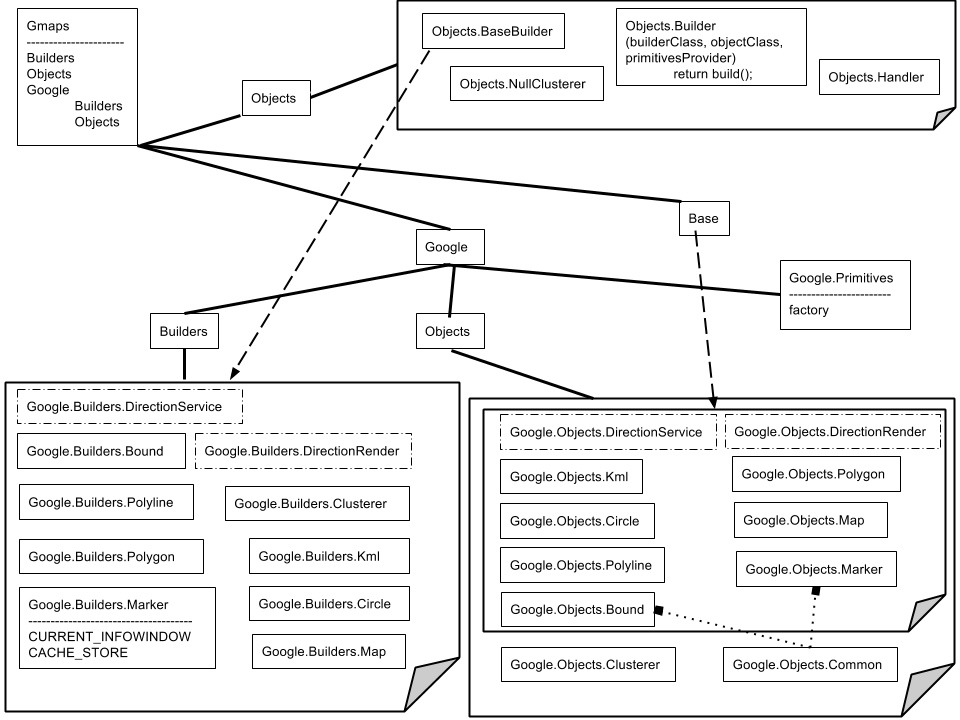
\includegraphics[scale=0.35]{images/novo_diagrama_de_heranca_google_maps_for_rails.png}
    \caption{Novo Diagrama de Herança Google-Maps-For-Rails}
    \label{fig:novo_diagrama_de_heranca_google_maps_for_rails}
  \end{center}  \
\end{figure}

Agora que acrescentamos estas quatro classes na gema adaptada, devemos adicionar no ‘‘\emph{Handler}'',
novas funções para manipular essas classes. E neste caso, inserimos as funçãoes ‘‘\emph{addDirection()}'' e
‘‘\emph{calculate\_route()}'' que podem ser vistas no algoritmo do código
\ref{lst:algoritmo_de_funcoes_adicionais_do_handler} que será explicado logo a seguir. A implementação deste
algoritmo está no apêndice \ref{chapter:codigos_ruby} no código \emph{Ruby}
\ref{lst:funcoes_adicionais_do_handler}.

\lstinputlisting[ style=customAlgoritmo, caption={Algoritmo de Funções adicionais do Handler}, label={lst:algoritmo_de_funcoes_adicionais_do_handler}]
{codigos/algoritmo_de_funcoes_adicionais_do_handler.coffee}

\begin{itemize}

 \item Na linha ‘‘1'' temos a definição da classe ‘‘\emph{Handler}''.

 \item Os ‘‘...'' representam os códigos já existentes na classe e que não são importantes para o
 exemplo.

 \item Na linha ‘‘3'' é adicionado a função ‘‘\emph{addDirection}'' que recebe como parâmetro
 ‘‘\emph{dados\_da\_direcao}'', que possui o informações do local de origem e local de destino que são
 obrigatórios para criar a direção, e as ‘‘\emph{opcoes}'' que pode conter as opções da forma
 como esse direção deve ser gerada. Essa função tem por objetivo criar as direções e colocá-las no mapas.

 \item Na linha ‘‘13'' é adicionado a função ‘‘\emph{calculate\_route}'' com o parâmetro
 ‘‘\emph{dados\_da\_direcao}'', que tem por principal objetivo fazer a requisição para o \emph{Google} de uma
 possível direção entre o local de origem ao local de destino.

\end{itemize}

Analisando as modificações, percebemos que somente inserimos 4 classes e 2 funções. Com isso podemos
perceber que as alterações que fizemos, não afetaram o funcionamento da gema, pois não foi
necessário mexer no código que já existia.

Existem outras possíveis soluções, como por exemplo, a criação de somente uma função para criar e
requisitar direções ao \emph{Google}, e também poderiamos pensar em mesclar as direções com os
\emph{markers}, devido ao fato que as direçõs utilizam \emph{markers} para marcar o ponto de inicio e
o ponto de fim. No entanto, nenhuma das duas modificações é benéfica para a biblioteca, pois a primeira
não faz a modularização, e a segunda aumenta a complexidade da biblioteca.


\subsection{API da Biblioteca Adaptada}
\label{subsection:api_da_biblioteca_adaptada}


Para facilitar o uso da nova funcionalidade de direções, apresentaremos rapidamente nesta seção,
a \emph{API} da gema adaptada.

Basicamente a função adicionada é a \emph{addDirection()} que recebe como parâmetro um local de origem
e um local de destino. E depois de fazer a requisição ao \emph{Google}, retorna no mapa, o caminho entre
a origem e o destino.

\lstinputlisting[ style=customCoffee, caption={Exemplo CoffeeScript API Google-Maps-For-Rails Adaptado}, label={lst:exemplo_coffeescript_api_google-maps-for-rails_adaptado}]
{codigos/exemplo_coffeescript_api_google-maps-for-rails_adaptado.js.coffee}

Para utilizar a funcionalidade de direção da gema adaptada, basta fazer a instalação da gema. Depois incluir
a gema no projeto em que se deseja utilizar a funcionalidade de direções. Em seguida, dentro do projeto,
implementar o código de criar mapas que pode ser o mesmo usado na gema original.
E no fim para criar a direção, chamar a função \emph{addDirection()} com um local de origem e um local de destino.

O código \ref{lst:exemplo_coffeescript_api_google-maps-for-rails_adaptado}, mostra um código base para criar um
mapa com uma direção.


\subsection{Exemplo de Uso da Biblioteca Adaptada}
\label{subsection:exemplo_de_uso_da_biblioteca_adaptada}

Esta seção tem o objetivo de mostrar a utilização da gema de exemplo ‘‘\emph{Google-Maps-for-Rails}'',
que adaptamos no tutorial, em um projeto do \emph{framework Ruby On Rails}.

Como exemplo de uso da gema ‘‘\emph{Google-Maps-for-Rails}'' adaptada, criamos o projeto
‘‘\emph{\href{https://github.com/toshikomura/DiseasesMap}{DiseasesMap}}''
\footnote{DiseasesMap : \url{https://github.com/toshikomura/DiseasesMap}} que tem como objetivo representar
a frequência de doenças no mapa do \emph{Google}, utilizando sobreposições. Até o momento de término deste
trabalho, essa função ainda não havia sido implementada, mas mesmo assim, fizemos o uso da
funcionalidade de direções, somente para exemplificar o uso da gema modificada.

\lstinputlisting[ style=customCoffee, caption={Exemplo CoffeeScript que Cria Mapa com Direção}, label={lst:exemplo_coffeescript_que_cria_mapa_com_direcao}]
{codigos/DiseasesMap/app/assets/javascripts/locations.js.coffee}

Inicialmente fizemos a instalação e inclusão da gema adaptada no arquivo \emph{Gemfile} do projeto. Depois
criamos uma estrutura básica de \emph{model/view/controller} de ‘‘\emph{locations}''. E para fazer o uso
da função de direções utilizamos o código \ref{lst:exemplo_coffeescript_que_cria_mapa_com_direcao},
explicado logo abaixo.

\begin{itemize}

 \item Na linha ‘‘2'' é feita a preparação da estrutura de configuração do mapa com a chamada
 ‘‘\emph{GMaps.build('Google')}'', sendo feita a criação do \emph{objeto Handler}, que é atribuída a
 variável local ‘‘\emph{handler}'', juntamente com as outras configurações básicas que o mapa necessita.

 \item Na linha ‘‘3'' é feita a chamada de ‘‘\emph{handler.buildMap(...)}'' que tem como função, fazer a
 criação do mapa a parir das configurações básicas já definidas. No caso, estas configurações básicas
 são definidas quando é feita a chamada de ‘‘\emph{GMaps.build('Google')}''. São passados como parâmetros
 as variáveis, ‘‘\emph{provider}'' que no exemplo está vazio, e ‘‘\emph{internal}'' que define o ‘‘\emph{id}''
 do mapa como ‘‘\emph{map}''. Neste caso, o ‘‘\emph{id}'' serve para identificar o mapa a ser modificado.

 \item Na linha ‘‘7'' é criado uma \emph{function} determinada pelo símbolo ‘‘->''. Esta \emph{function}
 somente será executada depois que a função ‘‘\emph{handler.buildMap(...)}'' terminar, ou seja, quando a
 criação do mapa terminar.

 No exemplo do código essa função executa as seguintes operações:

  \subitem Na linha ‘‘8'' é feita a criação de um \emph{marker} com a chamada da função
  ‘‘\emph{handler.addMarker(...)}'', sendo passado como parâmetro, a sua posição que no caso é (0,0)
  definido ‘‘\emph{lat}'' e ‘‘\emph{lng}'', a sua imagem definida por ‘‘\emph{picture}'', e sua informação
  definido por ‘‘\emph{infowindow}''.

  \subitem Na linha ‘‘17'' é feita a extensão de fronteiras incluindo o novo \emph{marker} com a chamada
  da função ‘‘\emph{handler.bounds.extendWith(...)}'', sendo passado como parâmetro o \emph{marker} criado
  anteriormente.

  \subitem Na linha ‘‘19'' é feita a criação de direções com a chamada da função
  ‘‘\emph{handler.addDirection(...)}''que incluímos no ‘‘\emph{Handler}'', sendo passado como parâmetro, um
  local de origem definido por ‘‘\emph{ origin: ‘‘São Paulo''} '', e um local de destino definido por
  ‘‘\emph{destination: ‘‘Curitiba''} ''.

\end{itemize}

\lstinputlisting[ style=customRubyHTML, caption={Exemplo Locations view que Cria Mapa com Direção}, label={lst:exemplo_locations_view_que_cria_mapa_com_direcao}]
{codigos/index_simplificado.html.erb}

E para mostrar o mapa na view de ‘‘\emph{locations}'' adicionamos o código mostrado em
\ref{lst:exemplo_locations_view_que_cria_mapa_com_direcao}
que é parte do código da \emph{view}, explicado logo a seguir.

\begin{itemize}

 \item Na linha ‘‘1'' com a \emph{tag} \emph{<h1>...</h1>} é definido como título principal da \emph{view} o
 texto ‘‘\emph{Listining locations}''.

 \item Os ‘‘\emph{...}'' indica que existe código, mas por simplificação na explicação, ele não foi mostrado.

 \item Da linha ‘‘3'' a ‘‘5'' é definido uma \emph{div} com ‘‘800px'' de largura. Dentro dessa \emph{div},
 é definido o local para a criação do mapa com ‘‘800px'' de largura e ‘‘400px'' de altura. No caso, o local
 de criação do mapa, é referênciado pelo atributo \emph{id} que é o mesmo \emph{id} utilizado no código
 \ref{lst:exemplo_coffeescript_que_cria_mapa_com_direcao} na linha ‘‘10''.

\end{itemize}

Como resultado ao se acessar o \emph{index} de locations, obtemos como resultado a imagem
\ref{fig:caminho_entre_sao_paulo_e_curitiba}. Neste caso, a nossa gema adaptada com a nova funcionalidade
de direções, funcionou corretamente, pois o caminho mostrado é entre ‘‘São Paulo'' e ‘‘Curitiba'', como
requisitamos na linha ‘‘24'' do código \ref{lst:exemplo_coffeescript_que_cria_mapa_com_direcao}.

\begin{figure}[ht]
  \begin{center}
    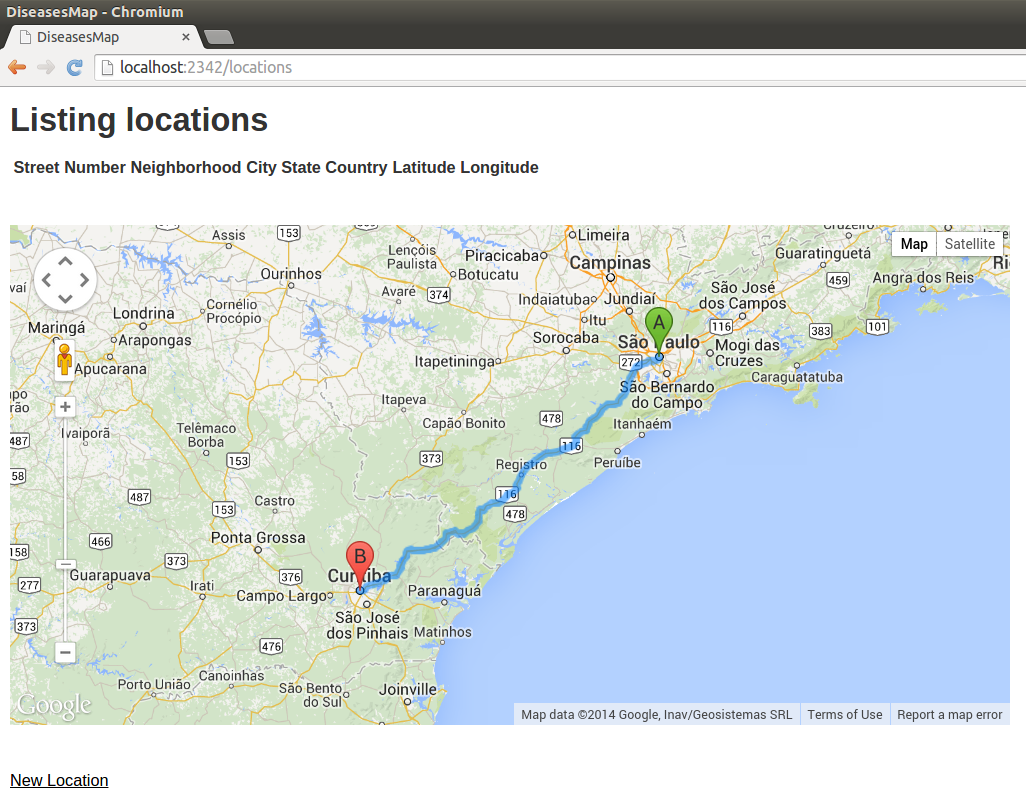
\includegraphics[scale=0.35]{images/caminho_entre_sao_paulo_e_curitiba.png}
    \caption{Caminho entre São Paulo e Curitiba}
    \label{fig:caminho_entre_sao_paulo_e_curitiba}
  \end{center}
\end{figure}
